%%%%%%%%%%%%%%%%%%%%%%%%%%%%%%%%%%%%%%%%%
% Journal Article
% LaTeX Template
% Version 1.3 (9/9/13)
%
% This template has been downloaded from:
% http://www.LaTeXTemplates.com
%
% Original author:
% Frits Wenneker (http://www.howtotex.com)
%
% License:
% CC BY-NC-SA 3.0 (http://creativecommons.org/licenses/by-nc-sa/3.0/)
%
%%%%%%%%%%%%%%%%%%%%%%%%%%%%%%%%%%%%%%%%%

%----------------------------------------------------------------------------------------
%	PACKAGES AND OTHER DOCUMENT CONFIGURATIONS
%----------------------------------------------------------------------------------------

\documentclass[twoside]{article}

\usepackage{lipsum} % Package to generate dummy text throughout this template

\usepackage[sc]{mathpazo} % Use the Palatino font
\usepackage[T1]{fontenc} % Use 8-bit encoding that has 256 glyphs
\usepackage[utf8]{inputenc}
\linespread{1.05} % Line spacing - Palatino needs more space between lines
\usepackage{microtype} % Slightly tweak font spacing for aesthetics
\usepackage{amsmath}

\usepackage[hmarginratio=1:1,top=32mm,columnsep=20pt]{geometry} % Document margins
\usepackage{multicol} % Used for the two-column layout of the document
\usepackage[hang, small,labelfont=bf,up,textfont=it,up]{caption} % Custom captions under/above floats in tables or figures
\usepackage{booktabs} % Horizontal rules in tables
\usepackage{float} % Required for tables and figures in the multi-column environment - they need to be placed in specific locations with the [H] (e.g. \begin{table}[H])
\usepackage{hyperref} % For hyperlinks in the PDF
\usepackage{multirow}

\usepackage{syntax}
\setlength{\grammarparsep}{5pt plus 1pt minus 1pt} % increase separation between rules
\setlength{\grammarindent}{6em} % increase separation between LHS/RHS 

\usepackage{lettrine} % The lettrine is the first enlarged letter at the beginning of the text
\usepackage{paralist} % Used for the compactitem environment which makes bullet points with less space between them

\usepackage{abstract} % Allows abstract customization
\renewcommand{\abstractnamefont}{\normalfont\bfseries} % Set the "Abstract" text to bold
\renewcommand{\abstracttextfont}{\normalfont\small\itshape} % Set the abstract itself to small italic text

\usepackage{pgf}
\usepackage{tikz}
\usetikzlibrary{arrows,automata, shapes, positioning, calc}

\newcommand{\rparen}{)}

\usepackage{titlesec} % Allows customization of titles
\renewcommand\thesection{\Roman{section}} % Roman numerals for the sections
\renewcommand{\thesubsection}{\thesection\hspace{1mm}\alph{subsection}}
\titleformat{\section}[block]{\large\scshape\centering}{\thesection}{1em}{} % Change the look of the section titles
\titleformat{\subsection}[block]{\large}{\thesubsection\rparen}{1em}{} % Change the look of the section titles

\usepackage{fancyhdr} % Headers and footers
\pagestyle{fancy} % All pages have headers and footers
\fancyhead{} % Blank out the default header
\fancyfoot{} % Blank out the default footer
\fancyhead[C]{TDT4205 Compilers $\bullet$ Assignment One $\bullet$ \date{\today}} % Custom header text
\fancyfoot[RO,LE]{\thepage} % Custom footer text

%----------------------------------------------------------------------------------------
%	TITLE SECTION
%----------------------------------------------------------------------------------------

\title{\vspace{-15mm}\fontsize{24pt}{10pt}\selectfont\textbf{Theory for Assignment Three}} % Article title

\author{
    \large
    \textsc{Øyvind Robertsen} \\ % Your name
    \normalsize Norwegian University of Science \& Technology \\ % Your institution
    \normalsize \href{mailto:oyvinrob@stud.ntnu.no}{oyvinrob@stud.ntnu.no} % Your email address
    \vspace{-5mm}
}
\date{}

%----------------------------------------------------------------------------------------

\begin{document}

\maketitle % Insert title

\thispagestyle{fancy} % All pages have headers and footers

%----------------------------------------------------------------------------------------
%	ABSTRACT
%----------------------------------------------------------------------------------------

%\begin{abstract}

%\noindent \lipsum[1] % Dummy abstract text

%\end{abstract}

%----------------------------------------------------------------------------------------
%	ARTICLE CONTENTS
%----------------------------------------------------------------------------------------

\begin{multicols}{2} % Two-column layout throughout the main article text

    \section{Problem 1}
    \subsection{Left factoring and eliminating left recursion}

    The first step is left factoring, resulting in the grammar in figure \ref{fig:prob1aleftfactored}.

    \begin{figure}[H]
        \begin{grammar}
            <A>     ::= g<A'>

            <A'>    ::= <B>
            \alt <C><D><E>

            <B>     ::= a
            \alt b<C>

            <C>     ::= c
            \alt $\epsilon$

            <D>     ::= <D>d
            \alt d

            <E>     ::= <E>e
            \alt d
        \end{grammar}
        \caption{Left factored grammar} \label{fig:prob1aleftfactored}
    \end{figure}

    Next up is eliminating left recursion.
    For the grammar in figure \ref{fig:prob1aleftfactored}, the $\langle D \rangle$ and $\langle E \rangle$ rules are the offending ones.
    The resulting grammar is listed in figure \ref{fig:prob1asolved}

    \begin{figure}[H]
        \begin{grammar}
            <A>     ::= g<A'>

            <A'>    ::= <B>
            \alt <C><D><E>

            <B>     ::= a
            \alt b<C>

            <C>     ::= c
            \alt $\epsilon$

            <D>     ::= d<D'>

            <D'>    ::= d<D'>
            \alt $\epsilon$

            <E>     ::= f<E'>

            <E'>    ::= e<E'>
            \alt $\epsilon$
        \end{grammar}
        \caption{Left recursion eliminated} \label{fig:prob1asolved}
    \end{figure}

    \newpage
    \subsection{FIRST and FOLLOW sets}

    FIRST sets first:

    \begin{gather*}
        \textrm{FIRST}(\langle A \rangle)   = \{ \textrm{g} \} \\
        \textrm{FIRST}(\langle A' \rangle)  = \{ \textrm{a, b, c, d} \} \\
        \textrm{FIRST}(\langle B \rangle)   = \{ \textrm{a, b} \} \\
        \textrm{FIRST}(\langle C \rangle)   = \{ \textrm{c, } \epsilon \} \\
        \textrm{FIRST}(\langle D \rangle)   = \{ \textrm{d} \} \\
        \textrm{FIRST}(\langle D' \rangle)  = \{ \textrm{d, } \epsilon \} \\
        \textrm{FIRST}(\langle E \rangle)   = \{ \textrm{f} \} \\
        \textrm{FIRST}(\langle E' \rangle)  = \{ \textrm{e, } \epsilon \}
    \end{gather*}

    Followed by FOLLOW sets:

    \begin{gather*}
        \textrm{FOLLOW}(\langle A \rangle)  = \{ \textrm{\$} \} \\
        \textrm{FOLLOW}(\langle A' \rangle) = \{ \textrm{\$} \} \\
        \textrm{FOLLOW}(\langle B \rangle)  = \{ \textrm{\$} \} \\
        \textrm{FOLLOW}(\langle C \rangle)  = \{ \textrm{\$, d} \} \\
        \textrm{FOLLOW}(\langle D \rangle)  = \{ \textrm{f} \} \\
        \textrm{FOLLOW}(\langle D' \rangle) = \{ \textrm{f} \} \\
        \textrm{FOLLOW}(\langle E \rangle)  = \{ \textrm{\$} \} \\
        \textrm{FOLLOW}(\langle E' \rangle) = \{ \textrm{\$} \} \\
    \end{gather*}

    \subsection{Predictive parsing table}

    The complete LL(1) predictive parsing table for the transformed grammar is given in table \ref{tab:prob1parsingtable}.

    \begin{table*}[t]
        \centering
        \begin{tabular}{l|l|l|l|l|l|l|l|l}
            ~           & a                 & b                 & c                 & d                         & e                 & f                         & g                 & \$                        \\ \hline
            \texttt{A}  & ~                 & ~                 & ~                 & ~                         & ~                 & ~                         & \texttt{A->gA'}   &  ~                        \\ \hline
            \texttt{A'} & \texttt{A'->B}    & \texttt{A'->B}    & \texttt{A'->CDE}  & \texttt{A'->CDE}          & ~                 & ~                         & ~                 &  ~                        \\ \hline
            \texttt{B}  & \texttt{B->a}     & \texttt{B->bC}    & ~                 & ~                         & ~                 & ~                         & ~                 &  ~                        \\ \hline
            \texttt{C}  & ~                 & ~                 & \texttt{C->c}     & \texttt{C->}$\epsilon$    & ~                 & ~                         & ~                 &  \texttt{C->}$\epsilon$   \\ \hline
            \texttt{D}  & ~                 & ~                 & ~                 & \texttt{D->dD'}           & ~                 & ~                         & ~                 &  ~                        \\ \hline
            \texttt{D'} & ~                 & ~                 & ~                 & \texttt{D->dD'}           & ~                 & \texttt{D'->}$\epsilon$   & ~                 &  ~                        \\ \hline
            \texttt{E}  & ~                 & ~                 & ~                 & ~                         & ~                 & \texttt{E->fE'}           & ~                 &  ~                        \\ \hline
            \texttt{E'} & ~                 & ~                 & ~                 & ~                         & \texttt{E'->eE'}  & ~                         & ~                 &  \texttt{E->}$\epsilon$   \\
        \end{tabular}
        \caption{LL(1) parsing table for the grammar in problem 1} \label{tab:prob1parsingtable}
    \end{table*}

    \subsection{Nonrecursive predictive parsing}

    The moves a predictive, nonrecursive parser would make on the input \texttt{gddfe} are given in table \ref{tab:prob1parsermoves}.

    \begin{table*}[t]
        \centering
        \begin{tabular}{l|r|r|l}
            Matched & Stack & Input & Action \\ \hline
            ~ & \texttt{A\$} & \texttt{gddfe\$} & ~ \\
            ~ & \texttt{gA'\$} & \texttt{gddfe\$} & output \texttt{A->gA} \\
            \texttt{g} & \texttt{A'\$} & \texttt{ddfe\$} & matched \texttt{g} \\
            \texttt{g} & \texttt{CDE\$} & \texttt{ddfe\$} & output \texttt{A'->CDE} \\
            \texttt{g} & \texttt{DE\$} & \texttt{ddfe\$} & output \texttt{C->}$\epsilon$ \\
            \texttt{g} & \texttt{dD'E\$} & \texttt{ddfe\$} & output \texttt{D->dD'} \\
            \texttt{gd} & \texttt{D'E\$} & \texttt{dfe\$} & matched \texttt{d} \\
            \texttt{gd} & \texttt{dD'E\$} & \texttt{dfe\$} & output \texttt{D'->dD'} \\
            \texttt{gdd} & \texttt{D'E\$} & \texttt{fe\$} & matched \texttt{d} \\
            \texttt{gdd} & \texttt{E\$} & \texttt{fe\$} & output \texttt{D'->}$\epsilon$ \\
            \texttt{gdd} & \texttt{fE'\$} & \texttt{fe\$} & output \texttt{E->fE'} \\
            \texttt{gddf} & \texttt{E'\$} & \texttt{e\$} & matched \texttt{f} \\
            \texttt{gddf} & \texttt{eE'\$} & \texttt{e\$} & output \texttt{E'->eE'} \\
            \texttt{gddfe} & \texttt{E'\$} & \texttt{\$} & matched \texttt{e} \\
            \texttt{gddfe} & \texttt{\$} & \texttt{\$} & output \texttt{E'->}$\epsilon$ \\ \hline
        \end{tabular}
        \caption{From top to bottom; the moves a predictive, nonrecursive parser for the grammar in problem 1 would make on the input \texttt{gddfe}.} \label{tab:prob1parsermoves}
    \end{table*}

    \section{Problem 2}
    \subsection{LR(0) automaton}

    The first step in creating the LR(0) automaton, is creating the augmented grammar. 
    The original grammar $G$ is augmented to the new grammar, $G'$, given in figure \ref{fig:prob2aaugmentedgrammar}.

    \begin{figure}[H]
        \begin{grammar}
            <A'>    ::= A

            <A>     ::= g<B>
            \alt g<C><D><E>

            <B>     ::= a
            \alt b<C>

            <C>     ::= c

            <D>     ::= <D>d
            \alt d

            <E>     ::= <E>e
            \alt f
        \end{grammar}
        \caption{Augmented grammar.} \label{fig:prob2aaugmentedgrammar}
    \end{figure}

    The canonical collection of sets is then computed according to the algorithm in figure $4.33$ in the Dragon Book.
    The first step is computing the closure of the set consisting only of the starting production.

    \begin{gather*}
        C = \{\textrm{CLOSURE}([\langle A' \rangle \rightarrow \cdot \langle A \rangle])\}
    \end{gather*}

    The initial set of items is given in figure \ref{fig:prob2ainitialclosure}.

    \begin{figure}[H]
        \centering
        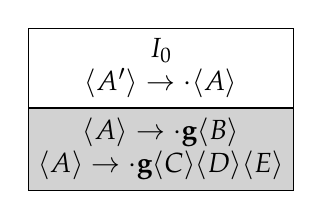
\begin{tikzpicture}
            [->, >=stealth', shorten >=1pt, auto, node distance=2.8cm, semithick,
            itemset/.style={rectangle split, rectangle split parts=2, rectangle split part fill={white, lightgray!70}, align=center, draw=black}]
            \node[itemset]      (I0)
            {$I_0$ \\
                $\langle A' \rangle \rightarrow \cdot \langle A \rangle$
                \nodepart{two}
                $\langle A \rangle \rightarrow \cdot \textbf{g} \langle B \rangle$ \\
                $\langle A \rangle \rightarrow \cdot \textbf{g} \langle C \rangle \langle D \rangle \langle E \rangle$
            };
        \end{tikzpicture}
        \caption{The result of computing the closure of the set consisting of the starting production.} \label{fig:prob2ainitialclosure}
    \end{figure}

    By adding sets of items computed by the GOTO function to the collection until no new sets can be added, we complete the canonical collection.
    The resulting automaton is show in figure \ref{fig:prob2aautomaton}.

    \begin{figure*}[t]
        \centering
        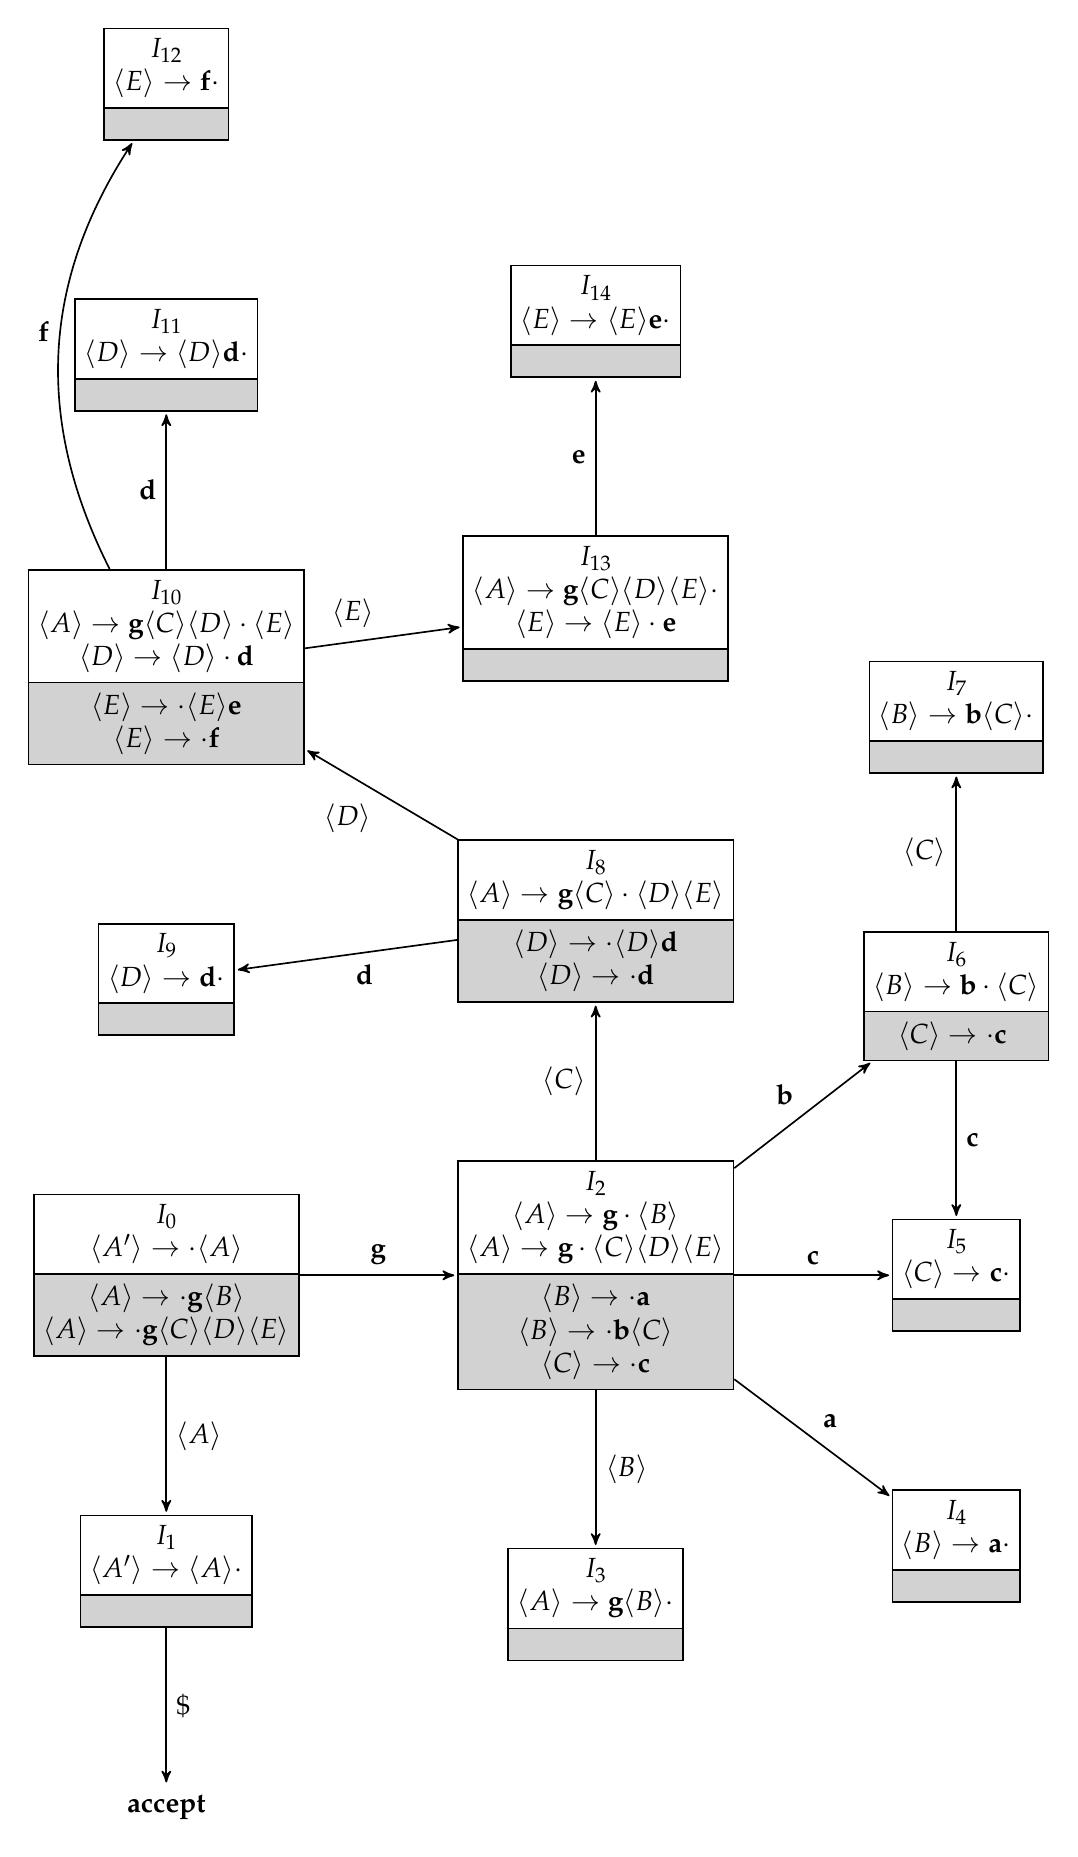
\begin{tikzpicture}
            [->, >=stealth', shorten >=1pt, auto, node distance=2cm, semithick,
            itemset/.style={rectangle split, rectangle split parts=2, rectangle split part fill={white, lightgray!70}, align=center, draw=black}]
            \node[itemset]  (I0)
            {$I_0$ \\
                $\langle A' \rangle \rightarrow \cdot \langle A \rangle$
                \nodepart{two}
                $\langle A \rangle \rightarrow \cdot \textbf{g} \langle B \rangle$ \\
                $\langle A \rangle \rightarrow \cdot \textbf{g} \langle C \rangle \langle D \rangle \langle E \rangle$
            };

            \node[itemset]  (I1)    [below = of I0]
            {$I_1$ \\
                $\langle A' \rangle \rightarrow \langle A \rangle \cdot$
            };
            
            \node[draw=none, fill=none]  (accept)    [below = of I1] {\textbf{accept}};

            \node[itemset]  (I2)    [right = of I0]
            {$I_2$ \\
                $\langle A \rangle \rightarrow \textbf{g} \cdot \langle B \rangle$ \\
                $\langle A \rangle \rightarrow \textbf{g} \cdot \langle C \rangle \langle D \rangle \langle E \rangle$
                \nodepart{two}
                $\langle B \rangle \rightarrow \cdot \textbf{a} $ \\
                $\langle B \rangle \rightarrow \cdot \textbf{b} \langle C \rangle$ \\
                $\langle C \rangle \rightarrow \cdot \textbf{c}$
            };

            \node[itemset]  (I3)    [below = of I2]
            {$I_3$ \\
                $\langle A \rangle \rightarrow \textbf{g} \langle B \rangle \cdot$
            };

            \node[itemset]  (I5)    [right = of I2]
            {$I_5$ \\
                $\langle C \rangle \rightarrow \textbf{c} \cdot$
            };

            \node[itemset]  (I4)    [below = of I5]
            {$I_4$ \\
                $\langle B \rangle \rightarrow \textbf{a} \cdot$
            };
            
            \node[itemset]  (I6)    [above = of I5]
            {$I_6$ \\
                $\langle B \rangle \rightarrow \textbf{b} \cdot \langle C \rangle$
                \nodepart{two}
                $\langle C \rangle \rightarrow \cdot \textbf{c}$
            };

            \node[itemset]  (I7)    [above = of I6]
            {$I_7$ \\
                $\langle B \rangle \rightarrow \textbf{b} \langle C \rangle \cdot$
            };

            \node[itemset]  (I8)    [above = of I2]
            {$I_8$ \\
                $\langle A \rangle \rightarrow \textbf{g} \langle C \rangle \cdot \langle D \rangle \langle E \rangle$
                \nodepart{two}
                $\langle D \rangle \rightarrow \cdot \langle D \rangle \textbf{d}$ \\
                $\langle D \rangle \rightarrow \cdot \textbf{d}$
            };

            \node[itemset]  (I9)    [above = of I0]
            {$I_9$ \\
                $\langle D \rangle \rightarrow \textbf{d} \cdot$
            };

            \node[itemset] (I10)   [above = of I9]
            {$I_{10}$ \\
                $\langle A \rangle \rightarrow \textbf{g} \langle C \rangle \langle D \rangle \cdot \langle E \rangle$ \\
                $\langle D \rangle \rightarrow \langle D \rangle \cdot \textbf{d}$
                \nodepart{two}
                $\langle E \rangle \rightarrow \cdot \langle E \rangle \textbf{e}$ \\
                $\langle E \rangle \rightarrow \cdot \textbf{f}$
            };

            \node[itemset]  (I11)   [above = of I10]
            {$I_{11}$ \\
                $\langle D \rangle \rightarrow \langle D \rangle \textbf{d} \cdot$
            };

            \node[itemset]  (I12)   [above = of I11]
            {$I_{12}$ \\
                $\langle E \rangle \rightarrow \textbf{f} \cdot $
            };

            \node[itemset]  (I13)   [above = of I8]
            {$I_{13}$ \\
                $\langle A \rangle \rightarrow \textbf{g} \langle C \rangle \langle D \rangle \langle E \rangle \cdot$ \\
                $\langle E \rangle \rightarrow \langle E \rangle \cdot \textbf{e}$
            };

            \node[itemset]  (I14)   [above = of I13]
            {$I_{14}$ \\
                $\langle E \rangle \rightarrow \langle E \rangle \textbf{e} \cdot$
            };

            \path (I0) edge                 node {$\langle A \rangle$}      (I1)
                  (I1) edge                 node {\$}                       (accept)
                  (I0) edge                 node {\textbf{g}}               (I2)
                  (I2) edge                 node {$\langle B \rangle$}      (I3)
                  (I2) edge                 node {\textbf{a}}               (I4)
                  (I2) edge                 node {\textbf{c}}               (I5)
                  (I2) edge                 node {\textbf{b}}               (I6)
                  (I6) edge                 node {\textbf{c}}               (I5)
                  (I6) edge                 node {$\langle C \rangle$}      (I7)
                  (I2) edge                 node {$\langle C \rangle$}      (I8)
                  (I8) edge                 node {\textbf{d}}               (I9)
                  (I8) edge                 node {$\langle D \rangle$}      (I10)
                  (I10) edge                node {\textbf{d}}               (I11)
                  (I10) edge [bend left]    node {\textbf{f}}               (I12)
                  (I10) edge                node {$\langle E \rangle$}      (I13)
                  (I13) edge                node {\textbf{e}}               (I14);
        \end{tikzpicture}
        \caption{The complete LR(0) automaton} \label{fig:prob2aautomaton}
    \end{figure*}

    \subsection{SLR parsing table}

    Computing ACTION($S$, $X$) for all states $S$ and all non-terminals $X$, as well as GOTO($S$, $Y$) for all states $S$ and nonterminals $Y$ yields the SLR parsing table (\ref{tab:prob2parsetable}).
    Inspired by the Dragon book, the following conventions are applied:

    \begin{itemize}
            \item s$i$ means shift and stack state $i$,
            \item r$j$ means reduce by the production numbered j,
            \item acc means accept,
            \item blank means error.
    \end{itemize}

    The production rules are numbered thusly:

    \begin{gather}
        \langle A \rangle ::= \textbf{g} \langle B \rangle \\
        \langle A \rangle ::= \textbf{g} \langle C \rangle \langle D \rangle \langle E \rangle \\
        \langle B \rangle ::= \textbf{a} \\
        \langle B \rangle ::= \textbf{b} \langle C \rangle \\
        \langle C \rangle ::= \textbf{c} \\
        \langle D \rangle ::= \langle D \rangle \textbf{d} \\
        \langle D \rangle ::= \textbf{d} \\
        \langle E \rangle ::= \langle E \rangle \textbf{e} \\
        \langle E \rangle ::= \textbf{f}
    \end{gather}

    \begin{table*}[b]
        \centering
        \begin{tabular}{|c|cccccccc|ccccc|}
            \hline
            \multirow{2}{*}{STATE} & \multicolumn{8}{|c|}{ACTION} & \multicolumn{5}{|c|}{GOTO} \\ \cline{2-14}
            ~ & \textbf{a} & \textbf{b} & \textbf{c} & \textbf{d} & \textbf{e} & \textbf{f} & \textbf{g} & \textbf{\$} & \textbf{A} & \textbf{B} & \textbf{C} & \textbf{D} & \textbf{E} \\ \hline
            0  & ~  & ~   & ~   & ~   & ~   & ~   & s2 & ~   & 1  & ~  & ~  & ~   & ~   \\ \hline
            1  & ~  & ~   & ~   & ~   & ~   & ~   & ~  & acc & ~  & ~  & ~  & ~   & ~   \\ \hline
            2  & s4 & s6  & s5  & ~   & ~   & ~   & ~  & ~   & ~  & 3  & 8  & ~   & ~   \\ \hline
            3  & ~  & ~   & ~   & ~   & ~   & ~   & ~  & r1  & ~  & ~  & ~  & ~   & ~   \\ \hline
            4  & ~  & ~   & ~   & ~   & ~   & ~   & ~  & r3  & ~  & ~  & ~  & ~   & ~   \\ \hline
            5  & ~  & ~   & ~   & r5  & ~   & ~   & ~  & ~   & ~  & ~  & ~  & ~   & ~   \\ \hline
            6  & ~  & ~   & s5  & ~   & ~   & ~   & ~  & ~   & ~  & ~  & 7  & ~   & ~   \\ \hline
            7  & ~  & ~   & ~   & ~   & ~   & ~   & ~  & r4  & ~  & ~  & ~  & ~   & ~   \\ \hline
            8  & ~  & ~   & ~   & s9  & ~   & ~   & ~  & ~   & ~  & ~  & ~  & 10  & ~   \\ \hline
            9  & ~  & ~   & ~   & ~   & ~   & r7  & ~  & ~   & ~  & ~  & ~  & ~   & ~   \\ \hline
            10 & ~  & ~   & ~   & s11 & ~   & s12 & ~  & ~   & ~  & ~  & ~  & ~   & 13  \\ \hline
            11 & ~  & ~   & ~   & ~   & ~   & r6  & ~  & ~   & ~  & ~  & ~  & ~   & ~   \\ \hline
            12 & ~  & ~   & ~   & ~   & r9  & ~   & ~  & r9  & ~  & ~  & ~  & ~   & ~   \\ \hline
            13 & ~  & ~   & ~   & ~   & s14 & ~   & ~  & ~   & ~  & ~  & ~  & ~   & ~   \\ \hline
            14 & ~  & ~   & ~   & ~   & ~   & ~   & ~  & r8  & ~  & ~  & ~  & ~   & ~   \\ \hline
        \end{tabular}
        \caption{SLR parse table for the grammar in problem 2} \label{tab:prob2parsetable}
    \end{table*}

    \subsection{SLR parsing moves}

    The moves done by an SLR parser on the input \texttt{gcddfe} using the parsing table constructed in the previous subtask are given in table \ref{tab:prob2parsemoves}.

    \begin{table*}[b]
        \centering
        \begin{tabular}{|r|l|l|r|l|}
            \hline
            ~    & Stack & Symbols & Input & Action \\ \hline
            (1)  & 0 & ~ & \textbf{gcddfe\$} & shift \\ \hline
            (2)  & 0 2 & \textbf{g} & \textbf{cddfe\$} & shift \\ \hline
            (3)  & 0 2 5 & \textbf{gc} & \textbf{ddfe\$} & reduce \textbf{C->c} \\ \hline
            (4)  & 0 2 8 & \textbf{gC} & \textbf{ddfe\$} & shift \\ \hline
            (5)  & 0 2 8 9 & \textbf{gCd} & \textbf{dfe\$} & reduce \textbf{D->d} \\ \hline
            (6)  & 0 2 8 10 & \textbf{gCD} & \textbf{dfe\$} & shift \\ \hline
            (7)  & 0 2 8 10 11 & \textbf{gCDd} & \textbf{fe\$} & reduce \textbf{D->Dd} \\ \hline
            (8)  & 0 2 8 10 & \textbf{gCD} & \textbf{fe\$} & shift \\ \hline
            (9)  & 0 2 8 10 12 & \textbf{gCDf} & \textbf{e\$} & reduce \textbf{E->f} \\ \hline
            (10) & 0 2 8 10 13 & \textbf{gCDE} & \textbf{e\$} & shift \\ \hline
            (11) & 0 2 8 10 13 14 & \textbf{gCDEe} & \textbf{\$} & reduce \textbf{E->Ee} \\ \hline
            (12) & 0 2 8 10 13 & \textbf{gCDE} & \textbf{\$} & reduce \textbf{A->gCDE} \\ \hline
            (13) & 0 1 & \textbf{A} & \textbf{\$} & accept \\ \hline
        \end{tabular}
        \caption{SLR parser moves on the input \textbf{gcddfe}.} \label{tab:prob2parsemoves}
    \end{table*}
\end{multicols}

\end{document}
